\chapter{New Revolutions in Particle Physics: Spontaneous Symmetry Breaking, Goldstone Bosons, and Gauge Invariance}

These notes follow Leonard Susskind's Lecture 7 in the supplementary \emph{Particle Physics 2: Standard Model} track, with curation by LazyingArt LLC. The lecture begins with a promise and a warning. The promise is that we are heading toward the question of how a photon-like particle can acquire mass. The warning is that we cannot begin with the Higgs mechanism itself. First we have to understand two technical ideas, and in the order Susskind insists on: spontaneous symmetry breaking and gauge invariance. The lecture is therefore preparatory in the best sense. It does not postpone the physics; it builds the language in which the physics can finally be stated sharply.

\section{The Road to a Massive Gauge Boson}

The central problem is simple to state. A gauge boson, such as the photon, appears to resist an ordinary mass term. If we write the mass down by hand, gauge invariance is lost. So we proceed indirectly. We begin with the more elementary question of how a symmetry can survive in the equations and yet fail to be respected by the ground state. Then we study the continuous case, where the broken symmetry leads not to domain walls but to massless excitations. Only after that are we ready to ask the sharper question: can the same \(U(1)\) symmetry be made local, with a phase that varies from point to point in spacetime?

This is exactly the order of the lecture. We first learn what spontaneous symmetry breaking means, first in a discrete system and then in a continuous one. We then learn what gauge invariance means, and why it demands an extra field. Only at the very end do these two stories begin to touch, and even there Susskind stops just before the full Higgs mechanism. The chapter should keep that deliberate incompleteness.

\section{Discrete Symmetry Breaking: Magnets, Explicit Bias, and the Domain Wall}

Susskind begins by reopening the previous lecture's magnetic model. Each little magnet may point either up or down, and neighboring spins lower the energy by being parallel. The crucial point is that there is no fundamental asymmetry between the two aligned states. The all-up state and the all-down state have the same energy. The underlying description is symmetric under
\[
\uparrow \longleftrightarrow \downarrow.
\]

Nevertheless, once the system has been cooled and all excess energy has been removed, it cannot remain neutral between these possibilities. It must settle into one or the other. A tiny perturbation far away is enough to choose the direction of the whole lattice. One frozen spin tells its neighbors how to save energy, those neighbors tell their neighbors, and the choice propagates outward. That is the first meaning of spontaneous symmetry breaking in the lecture: the equations are symmetric, but the ground state is not.

Susskind then immediately contrasts this with explicit symmetry breaking. Suppose we add a magnetic field pointing upward. Then the asymmetry is no longer produced by the ground state; it is already present in the energy function. A single spin by itself already prefers to point up. In that case the distinction between up and down is built in from the start, and a distant perturbation cannot overturn a macroscopic sample without paying a huge energy cost.

The lecture is careful about the word \emph{spontaneous}. It does not refer to a sudden dynamical flip, nor to the size of some derivative. It refers to the absence of a built-in preference, together with an instability of the ground state to arbitrarily small perturbations. At high temperature the system may contain a patchwork of up and down regions, but when it is cooled one orientation eventually wins. Which one wins is a matter of chance or of infinitesimal bias, not of a term in the fundamental energy that singles it out in advance.

\subsection{Question \& Answer}

\paragraph{Question.} How can we tell spontaneous symmetry breaking from explicit symmetry breaking?

\paragraph{Answer.} The lecture answers this operationally. Consider a large finite sample. Freeze the spins on the left boundary upward and freeze the spins on the right boundary downward. Then ask for the lowest-energy configuration in the bulk.

If the symmetry is explicitly broken, for example by a magnetic field favoring up everywhere, then the influence of the down boundary can only penetrate a short distance. To maintain a large region of down spins would cost an energy proportional to the size of that region. The interface is not stable in the middle.

If the symmetry is only spontaneously broken, then up and down are equally good in the bulk. In that case the lowest-energy configuration can contain one macroscopic region of up spins and one macroscopic region of down spins, separated by a transition region. That transition region is the domain wall. Its existence is the signal of the spontaneously broken discrete symmetry.

\begin{figure}[t]
\centering
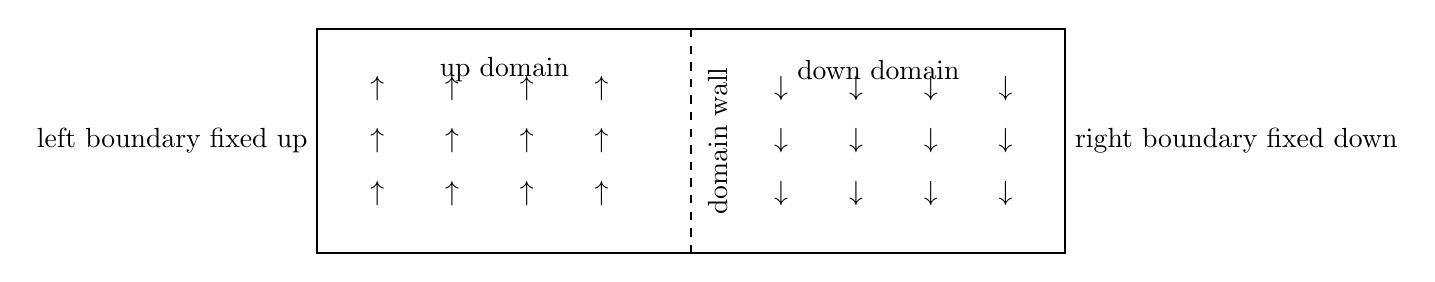
\begin{tikzpicture}[scale=0.95]
\draw[thick] (0,0) rectangle (10,3);
\draw[dashed,thick] (5,0) -- (5,3);
\node at (2.5,2.45) {up domain};
\node at (7.5,2.45) {down domain};
\node[rotate=90] at (5.35,1.5) {domain wall};
\foreach \x in {0.8,1.8,2.8,3.8}{
  \node at (\x,0.8) {$\uparrow$};
  \node at (\x,1.5) {$\uparrow$};
  \node at (\x,2.2) {$\uparrow$};
}
\foreach \x in {6.2,7.2,8.2,9.2}{
  \node at (\x,0.8) {$\downarrow$};
  \node at (\x,1.5) {$\downarrow$};
  \node at (\x,2.2) {$\downarrow$};
}
\node[left] at (0,1.5) {left boundary fixed up};
\node[right] at (10,1.5) {right boundary fixed down};
\end{tikzpicture}
\caption{Boundary conditions that reveal the discrete domain wall. In the spontaneously broken case both orientations are equally good in the bulk, so a macroscopic interface can survive.}
\label{fig:lecture07-domain-wall}
\end{figure}

\section{The Continuum Version: A Real Scalar Field}

Having made the idea concrete with magnets, the lecture changes language and says, in effect, now we can think of a field theory with the same behavior. Let \(\phi\) be a real scalar field. A clean relativistic reconstruction of the board discussion is
\begin{equation}
\mathcal{L}=\frac12\,\partial_\mu\phi\,\partial^\mu\phi - V(\phi).
\label{eq:real-scalar-lagrangian-refined}
\end{equation}
The corresponding energy density has the schematic form
\begin{equation}
\mathcal{E}=\frac12\,\dot{\phi}^{\,2}+\frac12\,(\nabla\phi)^2+V(\phi).
\label{eq:real-scalar-energy-refined}
\end{equation}

The symmetry is again discrete,
\[
\phi \longrightarrow -\phi.
\]
If the potential is symmetric and has degenerate minima at \(\phi=\pm f\), then there are two uniform ground states,
\[
\phi(x)=+f,
\qquad
\phi(x)=-f.
\]
This is the direct continuum analogue of the all-up and all-down magnetic states.

The lecture now poses the same question in field-theory form. Suppose we insist on \(\phi=+f\) on one side of space and \(\phi=-f\) on the other. Why can the field not jump abruptly? The answer is that a sharp jump produces a large gradient, and the gradient term in the energy punishes it. In one dimension the energetic cost is controlled by
\begin{equation}
E_{\text{grad}} \sim \int dx\,\frac12\left(\frac{d\phi}{dx}\right)^2.
\label{eq:wall-gradient-energy-refined}
\end{equation}
A sudden jump means a large derivative; a large derivative means a large energy. The field therefore interpolates across a finite transition region. The domain wall is not a discontinuity. It is a smooth but localized region in which the field moves from one minimum to the other.

This is the point at which the magnetic picture becomes field-theory language. The aligned spins of the lattice become a nearly constant field configuration, and the cost of misalignment becomes gradient energy. The argument is the same argument in a more flexible mathematical form.

The lecture also pauses to contrast this with the unbroken case. If the potential has a unique minimum at \(\phi=0\), then the vacuum simply sits at \(\phi=0\). Since \(\phi=0\) is already invariant under \(\phi\to-\phi\), the symmetry is not spontaneously broken.

One can also now see the continuum version of explicit breaking. If the double-well potential is tilted so that one side lies lower than the other, then the asymmetry is in the potential itself. The favored minimum is chosen already by the Lagrangian. In that case a domain wall is not stable in the middle of a large sample; it will move to wipe out the energetically disfavored region.

At this point Susskind makes the next transition explicit: everything we have discussed so far involves a discrete symmetry. But the symmetries of interest in particle physics, \(U(1)\), \(SU(2)\), and \(SU(3)\), are continuous. That is where the lecture now turns.

\section{A Very Specific Continuous Symmetry: The Complex Field and Global \(U(1)\)}

Rather than start with the most general group-theoretic story, the lecture narrows to the simplest representative example. Let \(\phi\) now be a complex field. Its value is not restricted to a line; it lives in an internal plane. We write
\begin{equation}
\phi=\phi_R+i\phi_I,
\qquad
\phi^*=\phi_R-i\phi_I,
\qquad
\phi^*\phi=\phi_R^2+\phi_I^2.
\label{eq:complex-components-refined}
\end{equation}
These are not components in physical space. They are the two real fields that together make up the complex field.

\begin{figure}[t]
\centering

\includegraphics[width=0.78\textwidth]{lecture_07_figure_02.png}
\caption{Complex field components and phase rotation on the \(\phi\)-plane. The board separates the component decomposition from the rotationally invariant combination \(\phi^*\phi\).}
\label{fig:lecture07-complex-board-refined}
\end{figure}

The kinetic term now becomes
\begin{equation}
\mathcal{L}=\partial_\mu\phi^*\,\partial^\mu\phi - V(\phi^*\phi).
\label{eq:complex-lagrangian-refined}
\end{equation}
The lecture treats this as the sum of the kinetic energies of \(\phi_R\) and \(\phi_I\), repackaged into complex notation. The symmetry is the global \(U(1)\) transformation
\begin{equation}
\phi' = e^{i\theta}\phi,
\qquad
\phi^{*\prime}=e^{-i\theta}\phi^*,
\label{eq:global-u1-refined}
\end{equation}
with \(\theta\) constant. The sign convention wobbles briefly on the board, but the mathematical content is stable: multiplying the field by a constant phase rotates it in the \((\phi_R,\phi_I)\)-plane.

\begin{figure}[t]
\centering
\begin{tikzpicture}[scale=1.1]
\draw[->] (-2.3,0) -- (2.6,0) node[right] {$\phi_R$};
\draw[->] (0,-2.1) -- (0,2.4) node[above] {$\phi_I$};
\draw[thick,->] (0,0) -- (1.55,0.9);
\draw[thick,->] (0,0) -- (1.15,1.4);
\draw[thick] (0.7,0) arc[start angle=0,end angle=38,radius=0.7];
\node at (0.95,0.32) {$\theta$};
\node[below right] at (1.55,0.9) {$\phi$};
\node[above right] at (1.15,1.4) {$e^{i\theta}\phi$};
\end{tikzpicture}
\caption{Clean internal-space picture of the global \(U(1)\) action: multiplication by a phase rotates the field in the \((\phi_R,\phi_I)\)-plane.}
\label{fig:lecture07-complex-tikz-refined}
\end{figure}

Because \(\theta\) is constant, the derivative transforms homogeneously:
\begin{equation}
\partial_\mu\phi' = e^{i\theta}\partial_\mu\phi,
\qquad
\partial_\mu\phi^{*\prime}=e^{-i\theta}\partial_\mu\phi^*.
\label{eq:global-derivative-transform}
\end{equation}
Hence
\[
\partial_\mu\phi^{*\prime}\,\partial^\mu\phi'
=
\partial_\mu\phi^*\,\partial^\mu\phi.
\]
Likewise, the potential remains invariant provided it depends only on \(\phi^*\phi\). That is why the lecture insists that the potential be a function of the rotationally invariant combination \(\phi^*\phi\), and not, say, of \(\phi_R\) alone.

Now the lecture compares two potentials. In the simplest unbroken case,
\begin{equation}
V(\phi^*\phi)=\phi^*\phi.
\label{eq:symmetric-paraboloid}
\end{equation}
The minimum lies at \(\phi=0\). Geometrically this is a paraboloid with its minimum at the origin, and the origin itself is invariant under rotation. So there is no spontaneous breaking.

The broken case is the quartic potential
\begin{equation}
V(\phi^*\phi)=-a\,\phi^*\phi+b(\phi^*\phi)^2,
\qquad a,b>0.
\label{eq:mexican-hat-refined}
\end{equation}
Near the origin the negative quadratic term drives the field away from zero; for large field values the positive quartic term stabilizes it. The minimum therefore lies on a circle,
\begin{equation}
\phi^*\phi=f^2.
\label{eq:vacuum-circle-refined}
\end{equation}
The potential remains rotationally symmetric, but the vacuum must choose one point on the circle. This is spontaneous breaking of a continuous symmetry.

\subsection{Question \& Answer}

\paragraph{Question.} Are there domain walls for a continuously broken symmetry?

\paragraph{Answer.} The lecture asks exactly this. We take a large sample, fix the field to point in direction \(A\) at one end, and in direction \(B\) at the other. In the discrete case the choice was between a sharp jump and no jump. Here there is a new possibility: the field may move continuously around the vacuum circle from \(A\) to \(B\).

A sudden transition is energetically bad because it makes the gradients large. A smooth interpolation is much cheaper because it stays on the vacuum track and spreads the gradient cost out over a long distance. Unless \(A\) and \(B\) are exactly diametrically opposite, one arc of the circle is shorter than the other, and that is the preferred path. Susskind remarks that one can justify the linear interpolation of the angle by a calculus-of-variations argument; the essential point is that the continuously broken symmetry replaces the domain wall by a smooth low-energy variation.

\begin{figure}[t]
\centering
\begin{tikzpicture}[scale=0.95]
\begin{scope}
\draw[->] (-3.2,0) -- (3.2,0) node[right] {$x$};
\fill (-2.7,0) circle (1.3pt);
\fill (2.7,0) circle (1.3pt);
\node[below] at (-2.7,0) {$x_L$};
\node[below] at (2.7,0) {$x_R$};
\draw[thick] (-2.7,1.15) .. controls (-1.4,1.15) and (0.1,0.65) .. (1.4,0.15) .. controls (2.0,-0.05) and (2.45,-0.02) .. (2.7,0.1);
\node at (-1.85,1.52) {$\alpha(x)$};
\end{scope}
\begin{scope}[xshift=8.2cm]
\draw (0,0) circle (2);
\fill (1.55,1.25) circle (1.4pt) node[above right] {$A$};
\fill (-0.55,1.92) circle (1.4pt) node[above] {$B$};
\draw[line width=1.2pt] (1.55,1.25) arc[start angle=39,end angle=106,radius=2];
\node at (0.95,2.35) {vacuum track};
\end{scope}
\end{tikzpicture}
\caption{Smooth interpolation for the continuously broken symmetry. Across space the angle changes gradually; in field space the motion follows the vacuum circle from \(A\) to \(B\).}
\label{fig:lecture07-smooth-interpolation-refined}
\end{figure}

\section{Goldstone Bosons: The Cheap Motion Along the Trough}

The next move in the lecture is the conceptual hinge of the whole chapter. If a field can change from one vacuum direction to another while staying on the vacuum track, then there is a kind of excitation which costs only gradient energy. What sort of particle does that correspond to?

Susskind answers by reminding us what \emph{massless} means from the point of view of wave motion. If a field varies like
\begin{equation}
\varphi(x)\sim e^{ikx},
\label{eq:plane-wave-refined}
\end{equation}
then \(k\) plays the role of momentum. If the energy of the mode tends to zero as \(k\to 0\), then the corresponding quanta have zero energy at zero momentum. That is the meaning of a massless particle in the lecture. A pure gradient mode has exactly this property: longer and longer wavelength means smaller and smaller gradient, and hence smaller and smaller energy.

So we now return to the broken complex field and rewrite it in polar variables,
\begin{equation}
\phi=\rho e^{i\alpha}.
\label{eq:polar-field-refined}
\end{equation}
Here \(\rho\) is the radial field and \(\alpha\) is the angular field. Both may vary from place to place and from time to time. Differentiating gives
\begin{align}
\partial_\mu\phi
&=
e^{i\alpha}\big(\partial_\mu\rho+i\rho\,\partial_\mu\alpha\big),
\label{eq:dphi-polar-refined}
\\
\partial_\mu\phi^*
&=
e^{-i\alpha}\big(\partial_\mu\rho-i\rho\,\partial_\mu\alpha\big).
\label{eq:dphistar-polar-refined}
\end{align}
When we multiply the two, the cross terms cancel:
\begin{equation}
\partial_\mu\phi^*\,\partial^\mu\phi
=
(\partial_\mu\rho)(\partial^\mu\rho)+\rho^2(\partial_\mu\alpha)(\partial^\mu\alpha).
\label{eq:polar-kinetic-refined}
\end{equation}
Thus the Lagrangian becomes, in the notation used on the board,
\begin{equation}
\mathcal{L}=(\partial\rho)^2+\rho^2(\partial\alpha)^2-V(\rho).
\label{eq:rho-alpha-lagrangian-refined}
\end{equation}
The last term should be read cautiously. The lecture and board use \(V(\rho)\) as shorthand after the change of variables, but the invariant statement is that the potential depends only on the radial degree of freedom, inherited from \(V(\phi^*\phi)=V(\rho^2)\). What matters is that \(\alpha\) does not appear in the potential.

\begin{figure}[t]
\centering

\includegraphics[width=0.88\textwidth]{lecture_07_figure_03.png}
\caption{Polar-field Lagrangian and symmetry-breaking potential as presented on the board. The boxed low-energy angular term and the Mexican-hat sketch appear together.}
\label{fig:lecture07-polar-board-refined}
\end{figure}

Now we make the low-energy approximation that drives the lecture. If we are interested only in very gentle excitations along the vacuum trough, then it does not pay to move radially away from the minimum. So we set
\[
\rho \approx f,
\]
where \(f\) is the vacuum radius. The lecture sometimes says \(F\); we standardize to \(f\). Then
\begin{equation}
\mathcal{L}_{\text{low }E}\approx f^2(\partial_\mu\alpha)(\partial^\mu\alpha).
\label{eq:low-energy-alpha-refined}
\end{equation}
Since \(f\) is just a constant, we can absorb it into the definition of the field:
\begin{equation}
\beta=f\alpha.
\label{eq:beta-definition-refined}
\end{equation}
This gives
\begin{equation}
\mathcal{L}_{\text{low }E}\approx (\partial_\mu\beta)(\partial^\mu\beta),
\label{eq:beta-massless-refined}
\end{equation}
up to conventional normalization. That is the Lagrangian of a massless field. The Goldstone boson is simply the quantum of the angular field, that is, the quantum of motion along the vacuum manifold.

\begin{figure}[t]
\centering
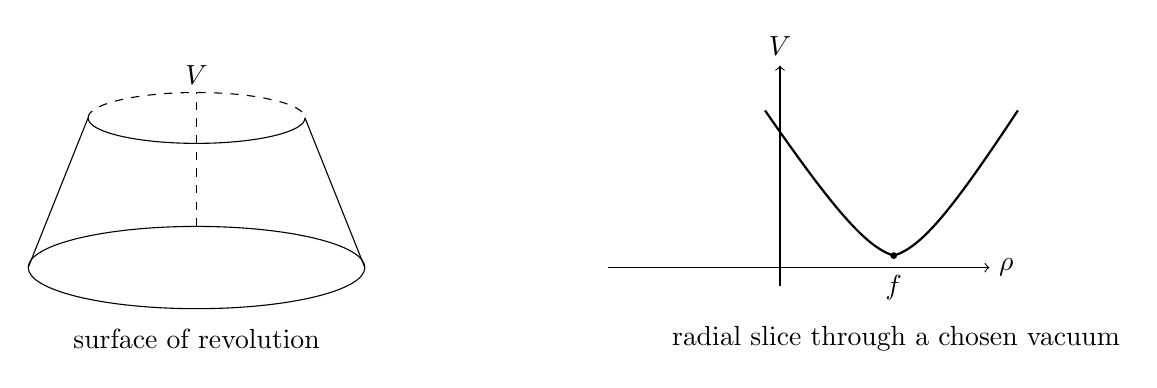
\begin{tikzpicture}[scale=0.95]
\begin{scope}
\draw (0,0) ellipse (2.25 and 0.55);
\draw (-2.25,0) -- (-1.45,2.0);
\draw (2.25,0) -- (1.45,2.0);
\draw (-1.45,2.0) arc[start angle=180,end angle=360,x radius=1.45,y radius=0.34];
\draw[dashed] (-1.45,2.0) arc[start angle=180,end angle=0,x radius=1.45,y radius=0.34];
\draw[dashed] (0,0.55) -- (0,2.35);
\node at (0,2.58) {$V$};
\node at (0,-0.95) {surface of revolution};
\end{scope}
\begin{scope}[xshift=7.8cm]
\draw[->] (-2.3,0) -- (2.8,0) node[right] {$\rho$};
\draw[->] (0,-0.25) -- (0,2.7) node[above] {$V$};
\draw[thick] (-0.2,2.1) .. controls (0.7,0.8) and (1.15,0.27) .. (1.52,0.16)
                         .. controls (1.9,0.27) and (2.32,0.8) .. (3.18,2.1);
\fill (1.52,0.16) circle (1.3pt);
\node[below] at (1.52,0.03) {$f$};
\node at (1.55,-0.95) {radial slice through a chosen vacuum};
\end{scope}
\end{tikzpicture}
\caption{Clean reconstruction of the symmetry-breaking potential: a circular trough of minima and a radial slice showing the restoring force in the \(\rho\) direction.}
\label{fig:lecture07-mexican-hat-refined}
\end{figure}

The two physically different modes are now easy to describe. If we displace the field along the circle, there is no restoring force. Only gradients cost energy, so the mode is massless. If we displace the field radially, the potential pulls it back toward the trough. A homogeneous radial displacement oscillates with nonzero frequency, and that nonzero zero-momentum oscillation energy is what the lecture interprets as a mass.

At this point Susskind broadens the notion of the Goldstone mode by analogy. Spin waves in a ferromagnet are Goldstone bosons of broken rotational symmetry. A long elastic string has a translation symmetry in the transverse direction if gravity is neglected; its very long wavelength transverse waves are Goldstone modes of that translation symmetry. A slinky or an ordinary compressible medium supports sound waves for essentially the same reason: a uniform translation of all molecules costs no energy, and a very slow translation that varies from place to place costs very little.

\begin{figure}[t]
\centering

\includegraphics[width=0.68\textwidth]{lecture_07_figure_04.png}
\caption{Long-wavelength Goldstone-wave sketch used in the discussion of spin waves and related analogies.}
\label{fig:lecture07-wave-board-refined}
\end{figure}

\begin{figure}[t]
\centering
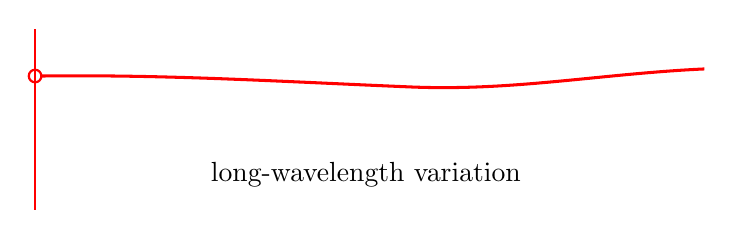
\begin{tikzpicture}[scale=1.0]
\draw[red,thick] (0,0) -- (0,2.3);
\draw[red,thick] (0,1.7) circle (0.08);
\draw[red,line width=1.1pt] (0.08,1.7)
  .. controls (1.7,1.72) and (3.1,1.63) .. (4.8,1.56)
  .. controls (6.1,1.51) and (7.2,1.73) .. (8.5,1.79);
\node at (4.2,0.45) {long-wavelength variation};
\end{tikzpicture}
\caption{A clean schematic of the slowly varying profile emphasized in the lecture: when the variation is spread over a long distance, the energy cost becomes small.}
\label{fig:lecture07-wave-tikz-refined}
\end{figure}

All of these examples share the same structure. There is a symmetry transformation that costs no energy when performed uniformly, and therefore its very gradual position-dependent version costs only a little energy. That is the mechanism behind Goldstone bosons.

\section{The Same \(U(1)\), Now Made Local}

The lecture now pivots, but not to a completely different subject. It is the same \(U(1)\) symmetry, only sharpened. Up to now \(\theta\) has been constant. But in a gauge theory we ask more: may the phase rotation vary from point to point?

Susskind frames this as a test. If we want to know whether a transformation is a symmetry, we apply it to the fields and substitute the transformed fields back into the Lagrangian. If the Lagrangian comes back unchanged, we have a symmetry. If not, we do not.

\subsection{Question \& Answer}

\paragraph{Question.} Can a local phase rotation be made into a symmetry?

\paragraph{Answer.} Not with ordinary derivatives alone. If the phase depends on spacetime, then differentiating the transformed field produces extra terms involving \(\partial_\mu\theta\). Those terms spoil the invariance of the kinetic term. The lecture's answer is to introduce a new field, the gauge field \(A_\mu\), and to redefine what we mean by differentiation. The symmetry can be restored, but only by enlarging the theory.

Let us carry out the test. Take
\begin{equation}
\phi'(x)=e^{i\theta(x)}\phi(x),
\label{eq:local-transform-refined}
\end{equation}
where \(\theta(x)\) is a spacetime-dependent symmetry parameter. It is not itself a dynamical field; it is the parameter of the transformation. Differentiating gives
\begin{align}
\partial_\mu\phi'
&=
e^{i\theta}\big(\partial_\mu\phi+i(\partial_\mu\theta)\phi\big),
\label{eq:dphi-prime-refined}
\\
\partial_\mu\phi^{*\prime}
&=
e^{-i\theta}\big(\partial_\mu\phi^*-i(\partial_\mu\theta)\phi^*\big).
\label{eq:dphistar-prime-refined}
\end{align}
Now the trouble is visible: the derivative of the transformed field is not just the transformed derivative of the original field. There is an extra piece proportional to \(\partial_\mu\theta\). Multiplying the transformed derivatives, we find
\begin{equation}
\partial_\mu\phi^{*\prime}\,\partial^\mu\phi'
=
\partial_\mu\phi^*\,\partial^\mu\phi
+i\big(\phi\,\partial_\mu\phi^*-\phi^*\,\partial_\mu\phi\big)\partial^\mu\theta
+\phi^*\phi\,\partial_\mu\theta\,\partial^\mu\theta.
\label{eq:local-failure-refined}
\end{equation}
This is exactly the disaster the lecture wants us to see. The potential \(V(\phi^*\phi)\) is still invariant, because \(\phi^*\phi\) does not change under multiplication by a phase. But the kinetic term is not invariant. That is why a global \(U(1)\) symmetry does not automatically become a local one.

The lecture's remedy is to introduce a new field \(A_\mu\), the gauge field. We then give it a transformation law chosen precisely so that the unwanted derivative-of-\(\theta\) term will be cancelled. The board checks the sign midstream, but a consistent convention is
\begin{equation}
A'_\mu=A_\mu-\partial_\mu\theta.
\label{eq:gauge-field-transform-refined}
\end{equation}
With this in hand we define the covariant derivatives
\begin{equation}
D_\mu\phi=\partial_\mu\phi+iA_\mu\phi,
\qquad
D_\mu\phi^*=\partial_\mu\phi^*-iA_\mu\phi^*.
\label{eq:covariant-derivatives-refined}
\end{equation}
The lecture emphasizes that this makes sense only because \(\phi\) is complex. For a real scalar field one would not want to add an explicitly imaginary quantity.

Now the cancellation can be seen directly:
\begin{align}
D_\mu\phi'
&=
\partial_\mu\phi'+iA'_\mu\phi'
\nonumber\\
&=
e^{i\theta}\big(\partial_\mu\phi+i(\partial_\mu\theta)\phi\big)
+i\big(A_\mu-\partial_\mu\theta\big)e^{i\theta}\phi
\nonumber\\
&=
e^{i\theta}\big(\partial_\mu\phi+iA_\mu\phi\big)
=
e^{i\theta}D_\mu\phi.
\label{eq:covariant-transform-refined}
\end{align}
Similarly,
\begin{equation}
D_\mu\phi^{*\prime}=e^{-i\theta}D_\mu\phi^*.
\label{eq:covariant-transform-conjugate-refined}
\end{equation}
So the phase factors once again cancel in the product. The gauge-invariant scalar part of the theory is therefore obtained by replacing ordinary derivatives with covariant ones.

\begin{figure}[t]
\centering

\includegraphics[width=0.84\textwidth]{lecture_07_figure_05.png}
\caption{Covariant derivatives and the assembled gauge-invariant gauge-field terms. The right board keeps the cleaned final formulas, while the left board preserves part of the intermediate phase-transformation work.}
\label{fig:lecture07-gauge-board-refined}
\end{figure}

The lecture then reminds us that a gauge field must also have its own dynamics. That is the Maxwell part. The field strength is
\begin{equation}
F_{\mu\nu}=\partial_\mu A_\nu-\partial_\nu A_\mu.
\label{eq:field-strength-refined}
\end{equation}
It is antisymmetric, its mixed time-space components give the electric field, and its space-space components give the magnetic field. The Maxwell Lagrangian is built from \(F_{\mu\nu}F^{\mu\nu}\), up to conventional signs and factors. A clean standard form for the full theory is therefore
\begin{align}
D_\mu\phi&=\partial_\mu\phi+iA_\mu\phi,
\nonumber\\
D_\mu\phi^*&=\partial_\mu\phi^*-iA_\mu\phi^*,
\nonumber\\
\mathcal{L}
&=
D_\mu\phi^*\,D^\mu\phi
-
V(\phi^*\phi)
-
\frac14 F_{\mu\nu}F^{\mu\nu}.
\label{eq:full-gauge-lagrangian-refined}
\end{align}
The board itself writes the final line more schematically, ending with \(+F^2\); the point of the lecture is gauge invariance, not normalization.

We should also check that \(F_{\mu\nu}\) is indeed gauge invariant:
\begin{align}
F'_{\mu\nu}
&=
\partial_\mu A'_\nu-\partial_\nu A'_\mu
\nonumber\\
&=
\partial_\mu\big(A_\nu-\partial_\nu\theta\big)
-
\partial_\nu\big(A_\mu-\partial_\mu\theta\big)
\nonumber\\
&=
F_{\mu\nu}
-\partial_\mu\partial_\nu\theta
+\partial_\nu\partial_\mu\theta
=
F_{\mu\nu}.
\label{eq:F-invariant-refined}
\end{align}
The cancellation uses only the equality of mixed partial derivatives. This is why the Maxwell term may be added without spoiling gauge invariance.

At the end of the lecture Susskind sharpens the central obstruction. There is one term we would very much like to add if we were trying to make a photon-like field massive:
\begin{equation}
\Delta\mathcal{L}_{\text{mass}}=\frac12 m^2 A_\mu A^\mu.
\label{eq:forbidden-mass-refined}
\end{equation}
But this term is forbidden, because
\[
A_\mu A^\mu \neq A'_\mu A^{\mu\prime}.
\]
A direct mass term for the gauge field is not gauge invariant. So a photon cannot simply be given a mass by hand.

And now the lecture reaches the point it has been aiming at from the first minute. The photon cannot have a mass. Or can it? Perhaps spontaneous symmetry breaking can do what a bare mass term cannot. That is the cliffhanger. Susskind tells us the answer right away, but postpones the derivation: if we spontaneously break the \(U(1)\) symmetry in the gauge-invariant theory, the Goldstone boson will disappear from the physical spectrum and the gauge field will acquire a mass. That is the Higgs phenomenon, and it belongs to the next lecture.

\section{Summary and the Next Step}

The lecture has now assembled the two pieces it promised at the beginning.

First, spontaneous symmetry breaking means that the equations may remain symmetric even while the ground state chooses among degenerate alternatives. In the discrete case this produces domain walls. In the continuous case it produces a vacuum manifold and, with it, a massless Goldstone mode corresponding to slow motion along that manifold.

Second, gauge invariance is stronger than global symmetry. A constant phase rotation is easy; a local phase rotation fails unless we enlarge the theory by introducing the gauge field \(A_\mu\) and replacing ordinary derivatives by covariant ones. Once we do that, we obtain a consistent gauge-invariant theory of charged matter coupled to a vector potential. But that same gauge invariance forbids the direct mass term \(\tfrac12 m^2 A_\mu A^\mu\).

So we end where Susskind wants us to end: with a paradox that is now mathematically precise. Continuous spontaneous symmetry breaking seems to give an unwanted Goldstone boson, while gauge invariance forbids a hand-made mass for the gauge boson. The Higgs phenomenon will resolve both difficulties at once. This lecture builds the problem carefully; the next one supplies the solution.